\newpage
\iffalse
For the evaluation section I would start by saying what you have been forced to do:
Remove all cryptographic messages and simplify stuff, like equality checks. Also the original pi-calculus model uses memory cells, and maybe there?s a better way to express this with a session type, for example using some concept of state.
Another thing that?s missing on the session type is a way to express the violation of a security property (session types are mainly concerned about correctness, but here we want to use them for security, so that?s something missing).
 \fi
\section{Evaluation}
With each topic now presented, we need to see how they all come together, to form the basis for the future thesis. As the thesis will focus mostly on session types and the TPM in a security related notion I will here demonstrate how these can be put together to form TPM commands with session types. To illustrate the TPM commands, the code of \citeauthor{DBLP:conf/csfw/DelauneKRS11} has been used for reference, and can be found in the appendix. In their example we find the commands:
\begin{spacing}{1}
\begin{itemize}
	\item \textit{Read}: Read the value of the PCR
	\item \textit{Quote}: Generate a certificate of an input value
	\item \textit{CreateWrapKey}: Create wrap key
	\item \textit{LoadKey2}: Loads wrap key
	\item \textit{CertifyKey}: Certifies a key
	\item \textit{Unbind}: Unbinds PCR value
	\item \textit{Seal}: Seals data
	\item \textit{Unseal}: Unseals data
	\item \textit{Extend}: Extends PCR value
\end{itemize}
\end{spacing}
\noindent On the next page, can be seen how each of these commands are constructed by session types. It should be noted, that in the process of constructing the commands, certain limitations were found within the expressivity of session types such as simplifying conditionals and what to do with cryptographic messages. The original pi-calculus model uses memory cells, which might allow for a better way to express this with session types, e.g. using some concept of state. Another thing session types are missing to model security protocols, is a way to express the violation of security properties, as session types are mainly concerned about correctness and thus missing the security part. These concerns are some of the main points for the motivation of writing the future thesis. 
%\subsection{TPM as Session Types}
\newpage
\noindent TPM $\rightarrow$ KeyStorage (parameters)\\
TPM $\rightarrow$ Alice : PrivateKey. rec a \\
\begin{spacing}{1}
$\left\{
\begin{tabular}{ l p{10cm} }
	\textit{Read}: & Alice $\rightarrow$ TPM(bitstring). PCR $\rightarrow$ TPM(pcr\_value). TPM $\rightarrow$ PCR(pcr\_value). TPM $\rightarrow$ Alice(pcr\_value). rec a \\ \\
	\textit{Quote}: & Alice $\rightarrow$ TPM(bitstring). PCR $\rightarrow$ TPM(pcr\_value). TPM $\rightarrow$ PCR(pcr\_value). TPM $\rightarrow$ Alice : CertPCR. rec a\\ \\
	\textit{CreateWrapKey}: & Alice $\rightarrow$ TPM(data). PCR $\rightarrow$ TPm(pcr\_value). TPM $\rightarrow$ PCR(pcr\_value). KeyTable $\rightarrow$ TPM : KeyLoaded. TPM $\rightarrow$ Alice(data). rec a\\ \\
	\textit{LoadKey2}: & Alice $\rightarrow$ TPM : LoadKey2. PCR $\rightarrow$ TPM(pcr\_value). TPM $\rightarrow$ PCR(pcr\_value). KeyTable $\rightarrow$ TPM : KeyLoaded. TPM $\rightarrow$ KeyTable : KeyLoaded. rec a\\
	\textit{CertifyKey}: & Alice $\rightarrow$ TPM(data) KeyTable $\rightarrow$ TPM : KeyLoaded. TPM $\rightarrow$ Alice : Cert. rec a \\ \\
	\textit{Unbind}: & Alice $\rightarrow$ TPM : unbind. PCR $\rightarrow$ TPM(pcr\_value). TPM $\rightarrow$ PCR(pcr\_value). KeyTable $\rightarrow$ TPM : KeyLoaded. TPM $\rightarrow$ Alice : adec(data). rec a\\ \\
	\textit{Seal}: & Alice $\rightarrow$ TPM : seal. PCR $\rightarrow$ TPM(pcr\_value). TPM $\rightarrow$ PCR(pcr\_value). KeyTable $\rightarrow$ TPM : KeyLoaded. TPM $\rightarrow$ Alice(data). rec a\\ \\
	\textit{Unseal}: & Alice $\rightarrow$ TPM : unseal. PCR $\rightarrow$ TPM(pcr\_value). TPM $\rightarrow$ PCR(pcr\_value). KeyTable $\rightarrow$ TPM : KeyLoaded. TPM $\rightarrow$ Alice : KeyLoaded. rec a\\ \\
	\textit{Extend}: & Alice $\rightarrow$ TPM : extend. PCR $\rightarrow$ TPM(pcr\_value). TPM $\rightarrow$ PCR(pcr\_value) : hpcr. rec a
\end{tabular}
\right\}.$
\bigbreak
\bigbreak
\noindent The reader will notice that a lot of the commands look very similar, which proves that lack of expressiveness in session types when used on security protocols.
\end{spacing}

%\begin{center}
%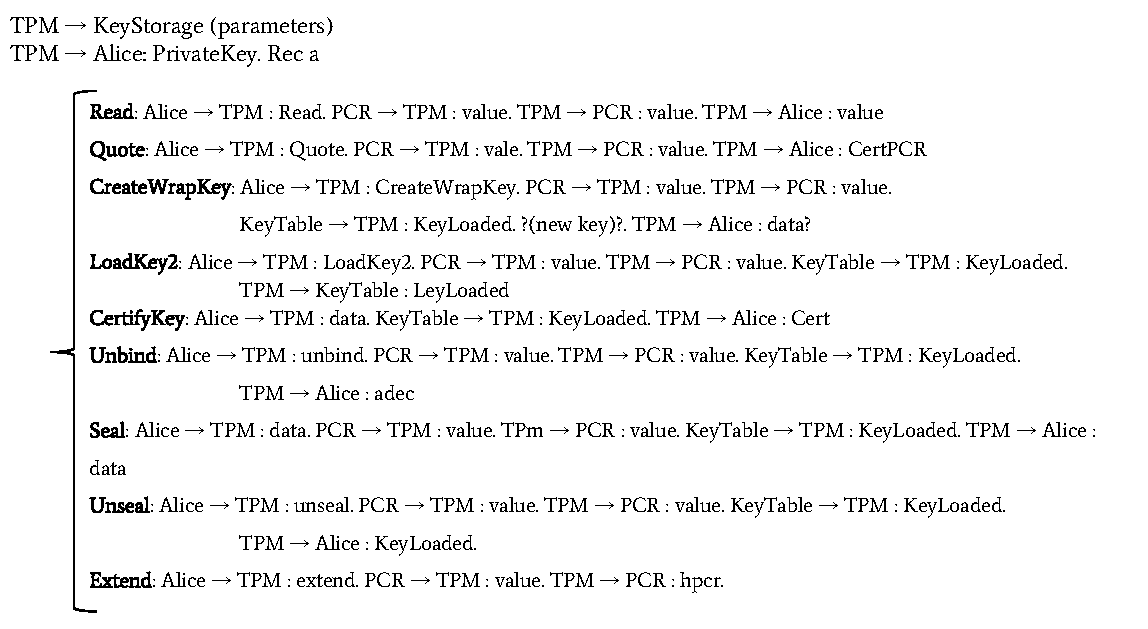
\includegraphics[width=1.2\textwidth, angle=0]{Graphics/Global_Types.pdf}
%\end{center}

%\noindent TODO: Description of above (+ code in appendix? for refs.)

% Extra
\iffalse
\begin{itemize}
  \item How they all come together
  \item Examples of TPM commands with session types
\end{itemize}
\fi

\iffalse
$\left\{
\begin{tabular}{ l }
	\textit{Read}: \enspace Alice $\rightarrow$ TPM : read. PCR $\rightarrow$ TPM : value. TPM $\rightarrow$ PCR : value.
	 \\ \hspace{4em} TPM $\rightarrow$ Alice : value. rec a \\
	\textit{Quote}: \enspace Alice $\rightarrow$ TPM : quote. PCR $\rightarrow$ TPM : value. TPM $\rightarrow$ PCR : value. 
	\\ \hspace{4em} TPM $\rightarrow$ Alice : CertPCR. rec a\\
	\textit{CreateWrapKey}: \enspace Alice $\rightarrow$ TPM : CreateWrapKey. PCR $\rightarrow$ TPm : value. 
	\\ \hspace{4em} TPM $\rightarrow$ PCR : value. KeyTable $\rightarrow$ TPM : KeyLoaded. \textbf{?(new key)?}. 
	\\ \hspace{4em} TPM $\rightarrow$ Alice : data. rec a\\
	\textit{LoadKey2}: \enspace Alice $\rightarrow$ TPM : LoadKey2. PCR $\rightarrow$ TPM : value. TPM $\rightarrow$ PCR : value. KeyTable $\rightarrow$ TPM : KeyLoaded. TPM $\rightarrow$ KeyTable : KeyLoaded. rec a\\
	\textit{CertifyKey}: \enspace Alice $\rightarrow$ TPM : data. KeyTable $\rightarrow$ TPM : KeyLoaded. TPM $\rightarrow$ Alice : Cert. rec a \\
	\textit{Unbind}: \enspace Alice $\rightarrow$ TPM : unbind. PCR $\rightarrow$ TPM : value. TPM $\rightarrow$ PCR : value. KeyTable $\rightarrow$ TPM : KeyLoaded. TPM $\rightarrow$ Alice : adec. rec a\\
	\textit{Seal}: \enspace Alice $\rightarrow$ TPM : data. PCR $\rightarrow$ TPM : value. TPM $\rightarrow$ PCR : value. KeyTable $\rightarrow$ TPM : KeyLoaded. TPM $\rightarrow$ Alice : data. rec a\\
	\textit{Unseal}: \enspace Alice $\rightarrow$ TPM : unseal. PCR $\rightarrow$ TPM : value. TPM $\rightarrow$ PCR : value. KeyTable $\rightarrow$ TPM : KeyLoaded. TPM $\rightarrow$ Alice : KeyLoaded. rec a\\
	\textit{Extend}: \enspace Alice $\rightarrow$ TPM : extend. PCR $\rightarrow$ TPM : value. TPm $\rightarrow$ PCR : hpcr. rec a
\end{tabular}
\right.$
\fi